%start by defining the document class
\documentclass[12pt]{article}

%below the package used for hyperlinking
\usepackage[a4paper, top=2.3cm, bottom=2.3cm, left=2.3cm, right=2.3cm]{geometry}
\usepackage{graphicx}	
\usepackage[brazil]{babel}
\usepackage{float}
\usepackage{hyperref}
\usepackage{amsfonts} 
\usepackage[brazil]{babel}
\graphicspath{ {../images/} }

\linespread{1.5}
\setlength{\parindent}{1.3cm}



%beggining of doc
\begin{document}

\begin{titlepage}
    \begin{center}
        \vspace*{1cm}
            
        \Huge
        \textbf{Simulação de Sinais Cerebrais de Espectroscopia por 
        Ressonância Magnética}
            
        \vspace{0.5cm}
        \LARGE
        Da Criação à Corrupção (Por Ruído)
            
        \vspace{1.5cm}
            
        \textbf{João Victor Dell Agli Floriano \\ Fernando Fernandes Paiva}

            
        \vfill
            
        \textbf{Curso:} Mestrado \\
        \textbf{Período a que se refere:} 02/2024 a 12/2024
            
        \vspace{0.8cm}
            
        \Large
        \textbf{Bolsa de Estudos:} CAPES \\
        \textbf{Período de Vigência:} 01/08/2024 a 28/02/2026 (19 meses)
            
    \end{center}
\end{titlepage}


%inserting the title defined above
% \maketitle
\section{Resumo do Projeto}

Muito embora o formalismo de Fourier tenha um retrospecto de sucesso no
processamento de sinais, existem situações nas quais a análise espectral utilizando
esse ferramental se torna bastante complicado. Para suprir essa demanda, alguns
algoritmos alternativos foram propostos nos últimos anos e, em particular, o método
matrix pencil (MPM, do inglês \textit{Matrix Pencil Method}) tem demonstrado seu potencial.
A possibilidade de se isolar cada uma das componentes do sinal original com base
em suas características únicas e avaliá-las independentemente deve permitir que
linhas pouco resolvidas atualmente possam ser analisadas com maior acurácia.
Esse tipo de análise ainda constitui um desafio para os métodos atuais de
processamento utilizados em dados de ressonância magnética e o MPM pode ser
um forte candidato a contribuir nesse sentido. O presente projeto propõe avaliar a
aplicabilidade do MPM para o processamento de dados clínicos de espectroscopia
por Espectroscopia por Ressonância Magnética (MRS, do inglês \textit{Magnetic Resonance Spectroscopy}). Este problema encontra uma série de aplicações na área clínica e os
métodos tradicionais ainda deixam a desejar, particularmente em situações nas
quais a resolução espectral é intrinsecamente baixa ou existe um alto grau de
superposição de informação.

\section{Cronograma Inicial}
\label{sec:cronograma}

Inicialmente, tinha-se como planejamento as seguintes etapas:

\begin{enumerate}
    \item  Etapa I: Estudo do algoritmo do MPM e obtenção dos créditos exigidos pelo
    Programa de Pós-Graduação referentes às disciplinas;
    \item  Etapa II: Desenvolvimento, implementação e validação do algoritmo e da
    rotina que simula dados complexos de RM;
    \item  Etapa III: Desenvolvimento, implementação e validação do algoritmo de
    processamento utilizando MPM;
    \item  Etapa IV: Estudo sistemático para determinação do efeito do ruído no
    processamento dos dados utilizando MPM;
    \item  Etapa V: Estudo da aplicabilidade do MPM para sinais de RM sintéticos e
    testes com dados de espectroscopia in vivo por RM;
    \item  Etapa VI: Redação da dissertação e defesa;
\end{enumerate}

E cronograma estabelecido:

\begin{table}[H] 
    \centering
    \begin{tabular}{|l|c|c|c|c|}
    \hline
    Etapas & Semestre 1 & Semestre 2 & Semestre 3 & Semestre 4 \\
    \hline
    I & X & X & & \\
    \hline
    II &  & X & & \\
    \hline
    III & & X & & \\
    \hline
    IV & & X & X &\\
    \hline
    V & & & X & X\\
    \hline
    VI & & & & X \\
    \hline
    \end{tabular}
    \caption{Cronograma do projeto}
    \label{table:2}
\end{table}

\section{Resumo do Presente Relatório}
No contexto das limitações apresentadas pelo formalismo de fourier, o MPM foi apresentado como uma 
alternativa de pós-processamento, visto que sua aplicação permite uma melhor separação das componentes 
de interesse do sinal.  Entretanto, o método ainda carece de limites bem definidos, particularmente no 
que se refere à aplicabilidade específica aos dados de Espectroscopia por Ressonância Magnética (MRS), 
nos quais o nível de ruído pode ser um desafio extra. Com o objetivo de investigar tais limites, foram 
implementadas rotinas para simulação de sinais sintéticos de MRS cerebral. Esses sinais foram então 
corrompidos com ruído de distribuição gaussiana, possibilitando o estudo de como diferentes valores de 
desvio padrão se comportavam nas várias etapas do processo de análise dos mesmos. Os primeiros resultados 
sugerem uma relação aproximadamente linear para valores mais baixos de ruído e uma saturação para valores 
mais altos. Os limites destes comportamentos, bem como sua caracterização para diferentes condições do sinal 
simulado, ainda estão sendo completamente caracterizados.


\section{Realizações no Período}
\subsection{Introdução}

A Ressonância Magnética (RM), inaugurada por meio do trabalho de Isidor Rabi em 1938 \cite{PhysRev.53.318} e 
posteriormente expandida por Felix Bloch e Edward Mills em 1946 \cite{Filler2009}, é uma das mais importantes e proeminentes áreas das
ciências físicas contemporâneas. Com subáreas que incluem Imageamento por Ressonância Magnética (MRI, do inglês \textit{Magnetic Resonance Imaging}) e 
MRS, sua aplicação nos estudos da saúde humana certamente contribuiu para
avanços significativos no aumento da expectativa de vida mundial, além de fornecer acesso a uma visão do corpo humano que antes
era vislumbrada apenas por meio de processos invasivos.

A MRS, domínio de interesse do presente trabalho, é uma subárea da RM que estuda espectros de resposta de compostos químicos. 
Esses espectros, por sua vez, tem uma ordem de grandeza de sinal menor se comparados aos sinais recebidos pelo MRI, que são emitidos 
principalmente por água e gordura. Suprimindo esses elementos de maior sinal, o estudo de tais compostos se torna possível. 
Essa subárea viabiliza exames da saúde de partes como o cérebro, que por meio da análise dos picos de resposta de cada composto, 
consegue verificar quantidades, as quais se comparadas a um exame saudável de referência, podem indicar distúrbios.

Apesar de se encontrar em um estágio avançado de compreensão, sendo pesquisada constantemente por centenas de grupos ao redor do mundo, a 
área geral de RM ainda carece de entendimento de alguns fenômenos, além de ter aplicação limitada por insuficiências de equipamento. 
Uma das insuficiências, caracterizada pela presença de ruído em sinais, pode afetar consideravelmente a capacidade de 
analisar de maneira efetiva sinais de espectroscopia para aplicação clínica. 

De maneira a mitigar os efeitos causados pelo ruído, especialmente no domínio da MRS, é sugerida a utilização do método MPM. O MPM é uma técnica numérica
de estimativa de parâmetros de sinais, desenvolvido originalmente por Yingbo Hua e Tapan Sakar \cite{370583} como uma alternativa a métodos já existentes 
como o de Prony \cite{49090}. O método consiste em modelar os sinais como uma soma de exponenciais complexas amortecidas, como na \autoref{eq:11}. Partindo 
dessa ideia, é então aplicada uma série de etapas, que inclui a utilização de outros métodos, como Decomposição em Valores Singulares (SVD, do inglês \textit{Singular Value Decomposition}), 
para estimar os parâmteros dessa função modeladora.  


\begin{equation} \label{eq:11}
    y(n) = \sum_{k=1}^{M} R_k e^{i (\omega_k t + \phi_k) + \alpha_k }
\end{equation}

Essa sugestão do MPM, apesar de inicialmente parecer deslocada da área de RM, tem seu motivo. Os sinais de RM medidos, por motivos a serem esclarecidos posteriormente, seguem o mesmo
formato da \autoref{eq:11}, justificando essa escolha.

\subsection{Métodos}

A fim de atingir o objetivo final de avaliação do MPM em sinais cerebrais de MRS, algumas etapas foram 
necessárias para que as condições ideais de testagem fossem estabelecidas. Para que esse algoritmo 
seja devidamente avaliado, é necessário primeiro garantir um total controle sobre as simulações as quais o mesmo estará submetido,
tornando essencial a caracterização do comportamento de variáveis dinâmicas, como por exemplo, a quantidade de ruído inserido no sinal final.


\subsubsection{Simulação}

Partindo desse objetivo, a primeira etapa do projeto foi a criação de um ambiente de simulação
que permitisse simular dados com diferentes durações, desvios químicos, configurações de ruído e amplitudes diferentes. Para a simulação, escrita em uma biblioteca 
própria customizada de python, foi escolhida uma abordagem mais analítica, considerando que o objeto de estudo seriam
sinais de MRS gerados a posteriori, e não o fenômeno físico em todos os seus detalhes. Sendo assim, foi simulada a evolução 
da equação básica de modelagem de um sinal de ressonância magnética, a solução transversal da equação de Bloch \cite{PhysRev.70.460}, 
descrita na \autoref{eq:1}.

\begin{equation} \label{eq:6}
    \mathbf{\frac{dM(t)}{dt}} = \mathbf{\gamma M(t)} \times \mathbf{B(t)}
\end{equation}

Quando resolvida, a \autoref{eq:6} rende a \autoref{eq:7} para a parte longitudinal, e a \autoref{eq:1} para a parte transversal.

\begin{equation} \label{eq:7}
    M_z(t) = M_0 (1 - e^{\frac{-t}{T_1}})
\end{equation}

\begin{equation} \label{eq:1}
    M_{xy}(t) = M_0 e^{i(\omega t + \phi)} e^{\frac{-t}{T_2}}
\end{equation}

A \autoref{eq:1} descreve a evolução da magnetização transversal de um conjunto de spins com magnetização inicial $M_0$, módulo da frequência de precessão $\omega$, fase inicial $\phi$ e tempo 
de relaxação transversal $T_2$. A figura \autoref{fig:3} demonstra um exemplo da evolução dessa equação no tempo, com 500 frequências sorteadas no intervalo de $(9.9, 10.1)$.  

\begin{figure} [H]
    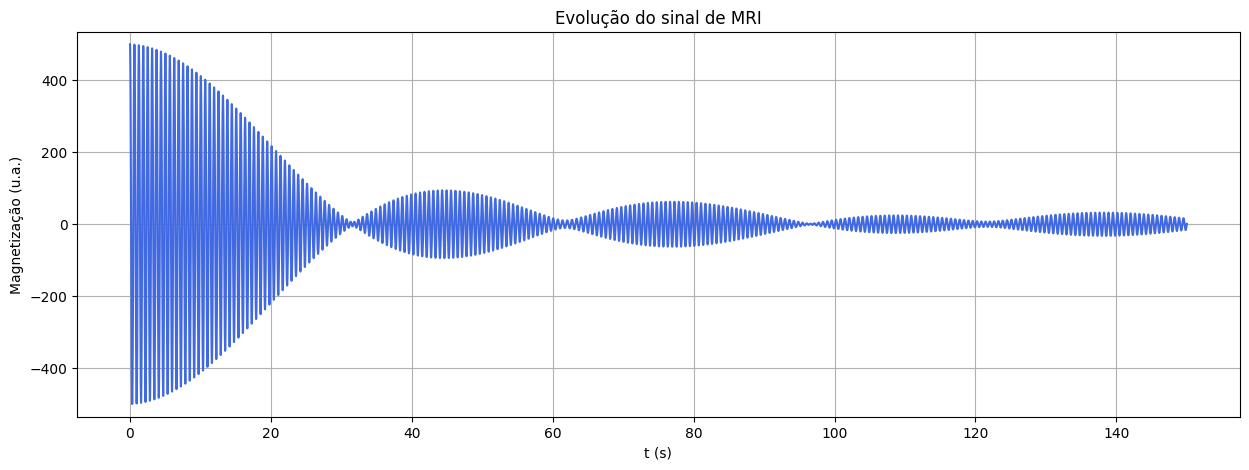
\includegraphics[scale=0.28]{sinal_simulado.png}
    \centering
    \caption{Resultado da simulação de decaimento da magnetização transversal para um conjunto de frequências.}
    \label{fig:3}
\end{figure}

O módulo da frequência de precessão é obtida a partir da razão giromagnética do núcleo alvo da ressonância, $\gamma$, e o campo magnético aplicado na amostra, $B_0$, através 
da equação de precessão de Larmor, descrita pela \autoref{eq:8}.

\begin{equation} \label{eq:8}
    |\mathbf{\omega}| = \gamma B_0
\end{equation}

No caso do núcleo de hidrogênio $H^1$, o alvo do procedimento de Ressonância Magnética Nuclear aqui simulado, a razão giromagnética é de $\gamma_H \approx 42,58 \ MHz/T$. O valor do tempo de relaxação transversal $T_2$ é 
mais empírica, que se origina da interação spin-spin do conjunto de spins sendo estudado. A interação entre os dipolos magnéticos acaba provocando uma perda de coerência de fase de precessão entre os mesmos, 
que emerge no decaimento do sinal de magnetização transversal medido.

A \autoref{fig:7} demonstra um exemplo dos tempos de relaxação longitudinal e transversal \cite{Mazzola_2015} para diferentes tecidos humanos, sob um campo de $1,5T$. 

\begin{figure}[H]
    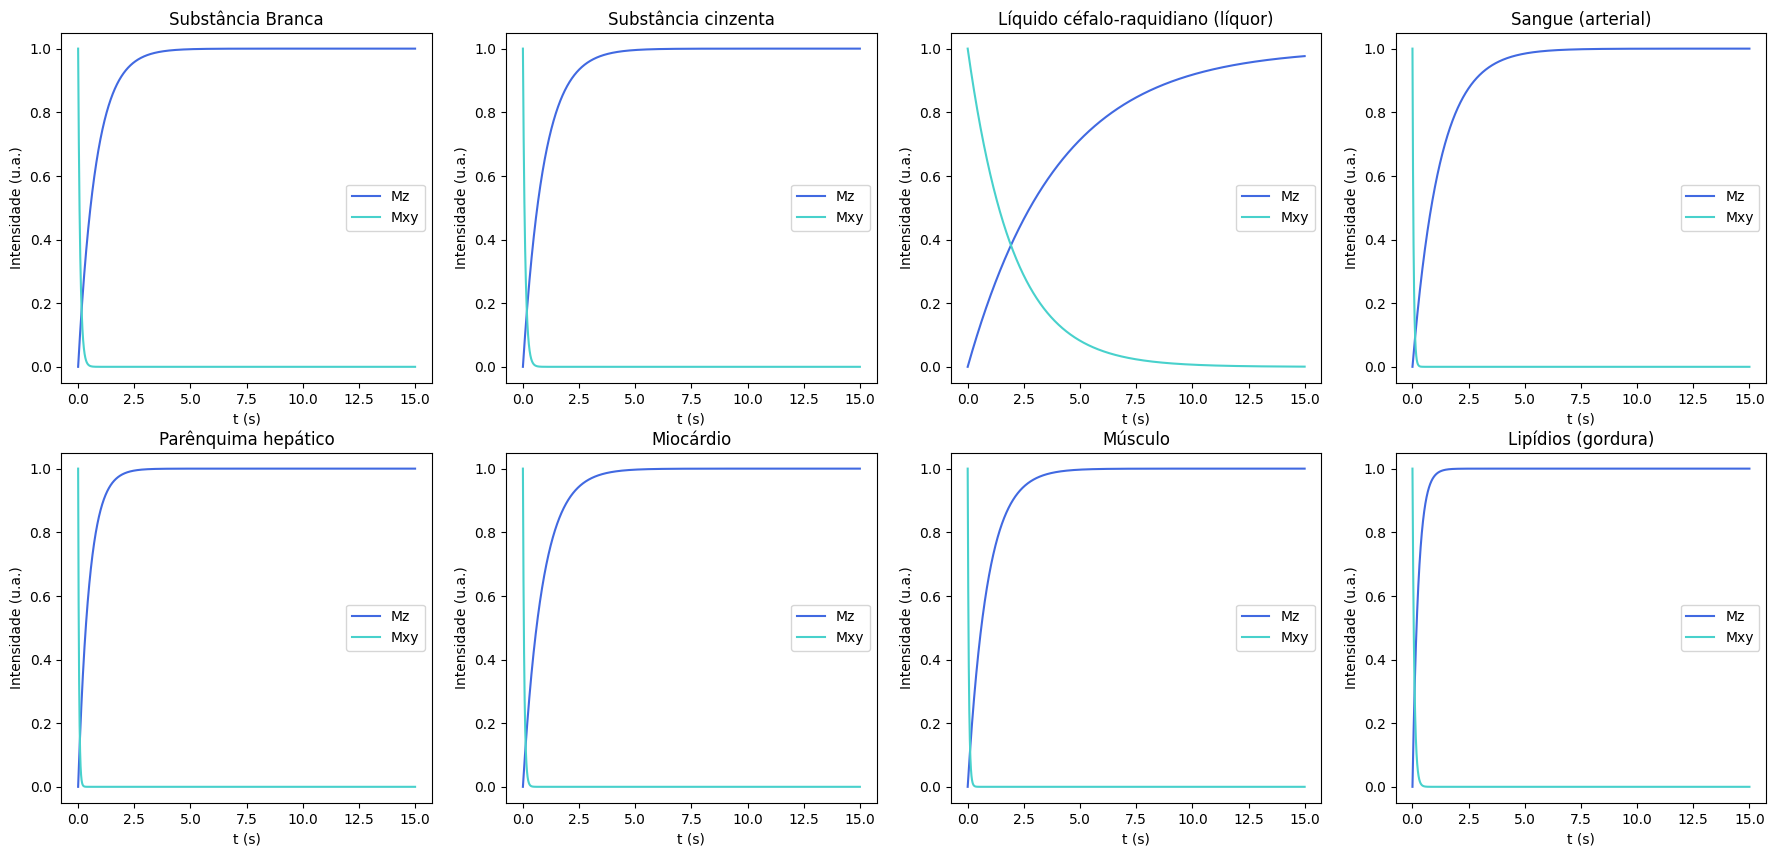
\includegraphics[scale=0.25]{T2.png}
    \centering
    \caption{Exemplo de decaimento das magnetizações longitudinal e transversal para vários tecidos humanos a partir do referncial girante.}
    \label{fig:7}
\end{figure}

\subsubsection{Metabólitos Cerebrais}
\label{sec:metabolites}

Com o estabelecimento dos instrumentos necessários para a simulação de sinais de MRS, foi possível então prosseguir para a próxima etapa:
a simulação de sinais cerebrais de MRS.

O procedimento de MRS, apesar de compartilhar dos mesmos procedimentos do MRI, possui objetivos 
diferentes. Enquanto o MRI se preocupa com uma imagem anatômica, ou seja, uma malha de voxels, a MRS se preocupa com a informação contida em apenas um voxel ou grupo 
reduzido de voxels, denominados \textit{voxel-of-interest} (VOI). O sinal obtido no VOI é analisado suprimindo os efeitos de lipídeos e água, restando 
apenas os sinais de ordem menor, relativos à ruído e a, principalmente, metabólitos. Metabólitos são moléculas orgânicas de forma e composição 
variadas, sendo essenciais em processos celulares. Por possuírem átomos de hidrogênio, os mesmos podem ser analisados utilizando RM, diferindo entre si por pequenos 
deslocamentos de frequência. Essa diferença, denominada deslocamento químico, é causada por efeitos eletrônicos de sua vizinhança química, que por meio de um efeito de blindagem, 
altera o valor do campo magnético efetivo sentido pelo núcleo, alterando assim sua frequência de ressonância. Visando uma padronização em aplicações clínicas, esse fenômeno é medido 
como o deslocamento relativo à um valor de referência de um composto, usualmente o Tetrametilsilano (TMS), e é representado na literatura pelo símbolo $\delta$. Seu cálculo é dado pela \autoref{eq:4}.

\begin{equation} \label{eq:4}
    \delta = \frac{\nu _{amostra} - \nu _{TMS}}{\nu _{TMS}}
\end{equation}

O desvio químico, medido dessa forma, é dado em partes por milhão (ppm). Esse formato é mais conveniente pois independe do campo magnético da medida, que varia signficativamente a depender das 
condições e categorias de análises clínicas a serem feitas localmente.

Para a simulação, foram escolhidos um conjunto de metabólitos comumente encontrados no cérebro, e também mensuráveis em ambiente clínico. Os parâmetros de desvio químico ($\delta$), tempo de relaxação 
transversal ($T_2$) e amplitude de tais compostos, sob regime de um campo $3T$, foram organizados na \autoref{table:1} \cite{Silva2020-io}.

\begin{table}[H] 
    \centering
    \begin{tabular}{|l|c|c|c|}
    \hline
    Metabólito & $\delta$ (ppm) & $T_2$ (s) & Amplitude (U.A.) \\
    \hline
    GABA & 1.9346 & 0.0199 & 0.2917 \\
    NAA & 2.0050 & 0.0735 & 0.4289 \\
    NAAG & 2.1107 & 0.0066 & 0.0290 \\
    Glx2 & 2.1157 & 0.0909 & 0.0184 \\
    GABA2 & 2.2797 & 0.0833 & 0.0451 \\
    Glu & 2.3547 & 0.1163 & 0.0427 \\
    Cr & 3.0360 & 0.0926 & 0.2026 \\
    Cho & 3.2200 & 0.1136 & 0.0776 \\
    M-Ins3 & 3.2570 & 0.1053 & 0.0202 \\
    M-Ins & 3.5721 & 0.1471 & 0.0411 \\
    M-Ins2 & 3.6461 & 0.2222 & 0.0150 \\
    Glx & 3.7862 & 0.0457 & 0.1054 \\
    Cr2 & 3.9512 & 0.04 & 0.2991 \\
    Cho+M-Ins & 4.1233 & 0.0088 & 0.8244 \\
    \hline
    \end{tabular}
    \caption{Informações dos metabólitos cerebrais selecionados para a utilização	na simulação.}
    \label{table:1}
\end{table}

A \autoref{fig:4} é um exemplo do espectro resultante da simulação dos dados de metabólitos mencionados, após análise de Fourier. A simulação foi feita com 100000 pontos,
no intervalo de tempo de $[0.0, 1.0)$, sob um campo de $3T$. 

\begin{figure} [H]
    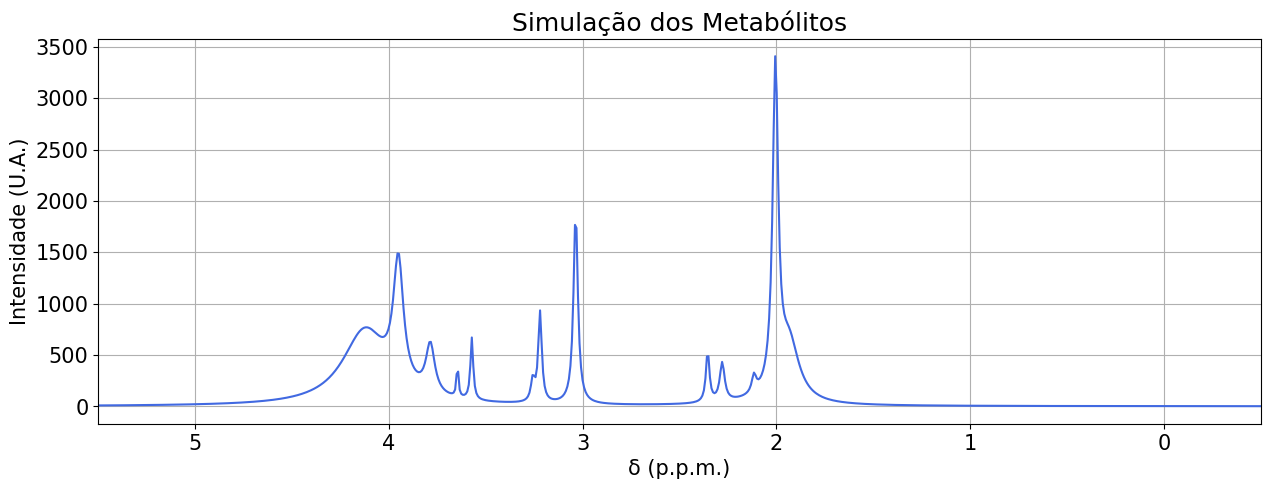
\includegraphics[scale=0.37]{metabolites.png}
    \centering
    \caption{Resultado da simulação dos metabólitos}
    \label{fig:4}
\end{figure}

\subsubsection{Adição de Ruído}
Apesar de o programa dar conta de simular espectros corretamente a partir dos parâmetros dados, a realidade é que sinais clínicos \textit{in vivo} tem uma aparência significativamente 
diferente da de um sinal gerado a partir do processo anteriormente descrito, principalmente por conta das distorções geradas por, por exemplo, alargamento de linha, ruído, entre outros. 

Os métodos de aquisição e conversão de sinais analógicos em digitais, por mais avançados que tenham se tornado se comparados à décadas passadas, ainda são limitados em vários aspectos. Uma das principais 
limitações ainda existentes é a captação de sinal ruidoso, o qual, a depender de sua intensidade, pode dificultar significativamente ou até impedir a análise do sinal desejado. A presença 
inevitável de ruído no sinal é, inclusive, uma das principais limitações que o MPM pretende enfrentar, tornando sua presença essencial neste estudo. 

No caso da maioria dos sinais captados, o ruído tem como distribuição geradora uma função gaussiana, definida pela \autoref{eq:3}. Nessa distribuição, $\mu$ representa seu valor central, 
que no caso do ruído captado por aparelhos, tem valor nulo. O segundo parâmetro, $\sigma$, representa a largura do intervalo de variação dos valores gerados a partir dessa 
distribuição, definido como sendo o valor adquirido na meia altura da curva, denominado desvio padrão.


\begin{equation} \label{eq:3}
    f(x) = \frac{1}{\sigma \sqrt{2\pi}}e^{-\frac{(x - \mu)^2}{2\sigma ^2}}
\end{equation}

Essa distribuição, definida em um módulo de números aleatórios da biblioteca \textit{numpy}, foi usada para geração de um ruído complexo, de mesmo $\sigma$ na parte real e imaginária, que foi então adicionado ao sinal original, simulando assim sua
corrupção.

Para fins de controle adequado da corrupção do sinal, a Relação Sinal-Ruído (SNR, do inglês \textit{Signal-to-noise Ratio}) foi usada como métrica de sua qualidade. O cálculo da SNR não possui uma definição unificada na literatura, podendo variar significativamente a depender da área. Sendo assim, 
escolheu-se a que seria mais conveniente para o contexto apresentado, atentando-se também a qual seria mais comum nos trabalhos de referência desse projeto. A definição a ser usada é a que 
leva em consideração o maior pico do espectro, representado por $P$, e o desvio padrão do ruído, representado por $\sigma$, como definido pela \autoref{eq:2}.  

\begin{equation} \label{eq:2}
    SNR = \frac{P}{\sigma}
\end{equation}

A \autoref{fig:5} demonstra a corrupção artificial do espectro, sob o ponto de vista de seu módulo, a partir de um $\sigma = 1.0$. Esse sinal variava 
entre o intevalo temporal de $[0.0, 1.0)$ segundos, com uma frequência de sampling de $100000$ pontos por segundo, resultando em $100000$ pontos.

\begin{figure} [H]
    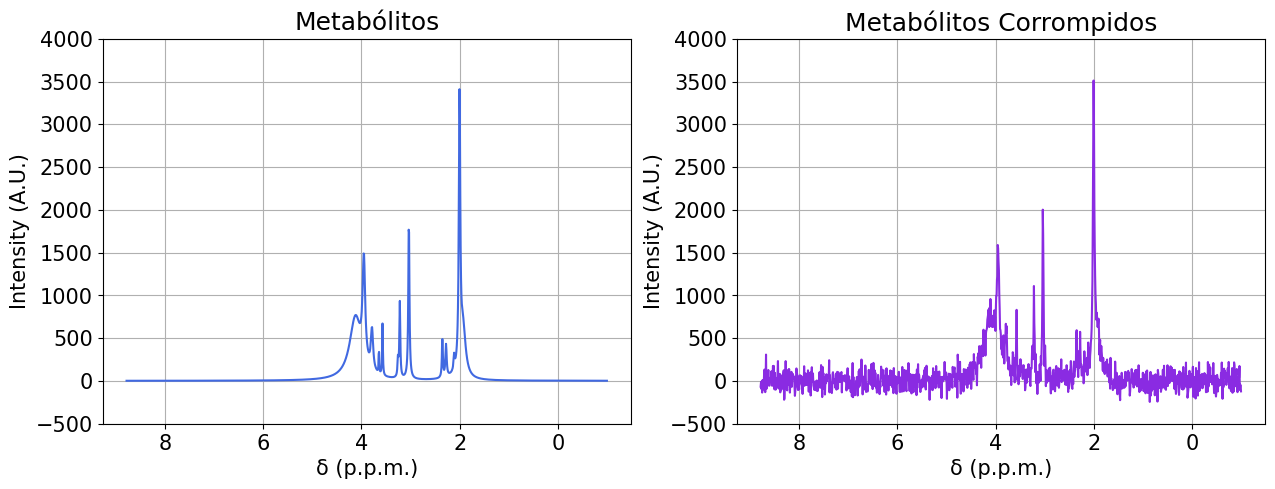
\includegraphics[scale=0.37]{metabolitos-corrompidos.png}
    \centering
    \caption{Comparação entre os metabólitos e sua versão corrompida}
    \label{fig:5}
\end{figure}

Para facilitar os cálculos, foi decidido normalizar o sinal gerado, dividindo-o pelo valor de seu pico, que se tornaria o valor de referência do sinal. O desvio padrão do ruído foi 
calculado, então, em uma região na qual se esperaria que o sinal predominante fosse de tal característica, que no caso dos metabólitos aqui simulados, se traduz na região final do sinal captado e do espectro, 
aqui definida como os últimos $10\%$ do espectro. 

\subsubsection{Relação entre desvios padrão}

Com o objetivo de obter maior controle da simulação, investigou-se o comportamento e a dependência entre o $\sigma$ utilizado para a geração de ruído na parte real e imaginária com o $\sigma$ resultante no módulo do espectro. A primeira abordagem 
tomada foi analítica, que a partir de definições estatísticas, não obteve sucesso na derivação de alguma relação direta. Optou-se então por uma abordagem experimental, na qual se gerou um conjunto de sinais 
corrompidos por desvios padrão de diferentes valores, e relacionou-os com suas partes resultantes no espectro, calculados por meio de sua definição 
estatística pela \autoref{eq:5}.

\begin{equation} \label{eq:5}
    \sigma = \sqrt{\frac{1}{N} \sum_{i=1}^{N} (x_i - \bar{x})^2}, \ com \ \bar{x} = \frac{1}{N} \sum_{i = 1}^{N} x_i  
\end{equation}

Essa investigação possibilitou a avaliação da implementação de uma função que, recebendo um valor desejado de SNR de entrada, forneceria qual deveria ser o valor aproximado do $\sigma$ usado pela distribuição 
geradora para que aquele valor de SNR fosse atingido, permitindo assim uma camada maior de controle dos parâmetros da simulação.

\subsection{Resultados e Discussão}

Para investigar a relação descrita, foram definidos limites dentro dos quais o desvio padrão usado na geração seria variado. Para isso foram gerados alguns sinais, baseando-se no espectro de metabólitos descritos na \autoref{sec:metabolites} com $\sigma$ variando inicialmente em um intervalo de $(0, 7)$, e calculados suas SNRs.
Comparando os valores calculados com exemplos reais de espectros cerebrais publicados na literatura, concluiu-se que os limites de ruído estavam excedendo os valores comumente encontrados. Além desse fator, como pode ser verificado pela figura \autoref{fig:9}, o intervalo de $\sigma$ o qual um sinal pode ser compreendido como tal, e não apenas ruído, seria aproximadamente $(0, 3)$. Para aumentar a precisão de um ajuste de parâmetros da 
curva resultante a ser feito posteriormente, o limite superior foi aumentado para $5$, se tornando então o intervalo final de $(0, 5)$.

\begin{figure}[H]
    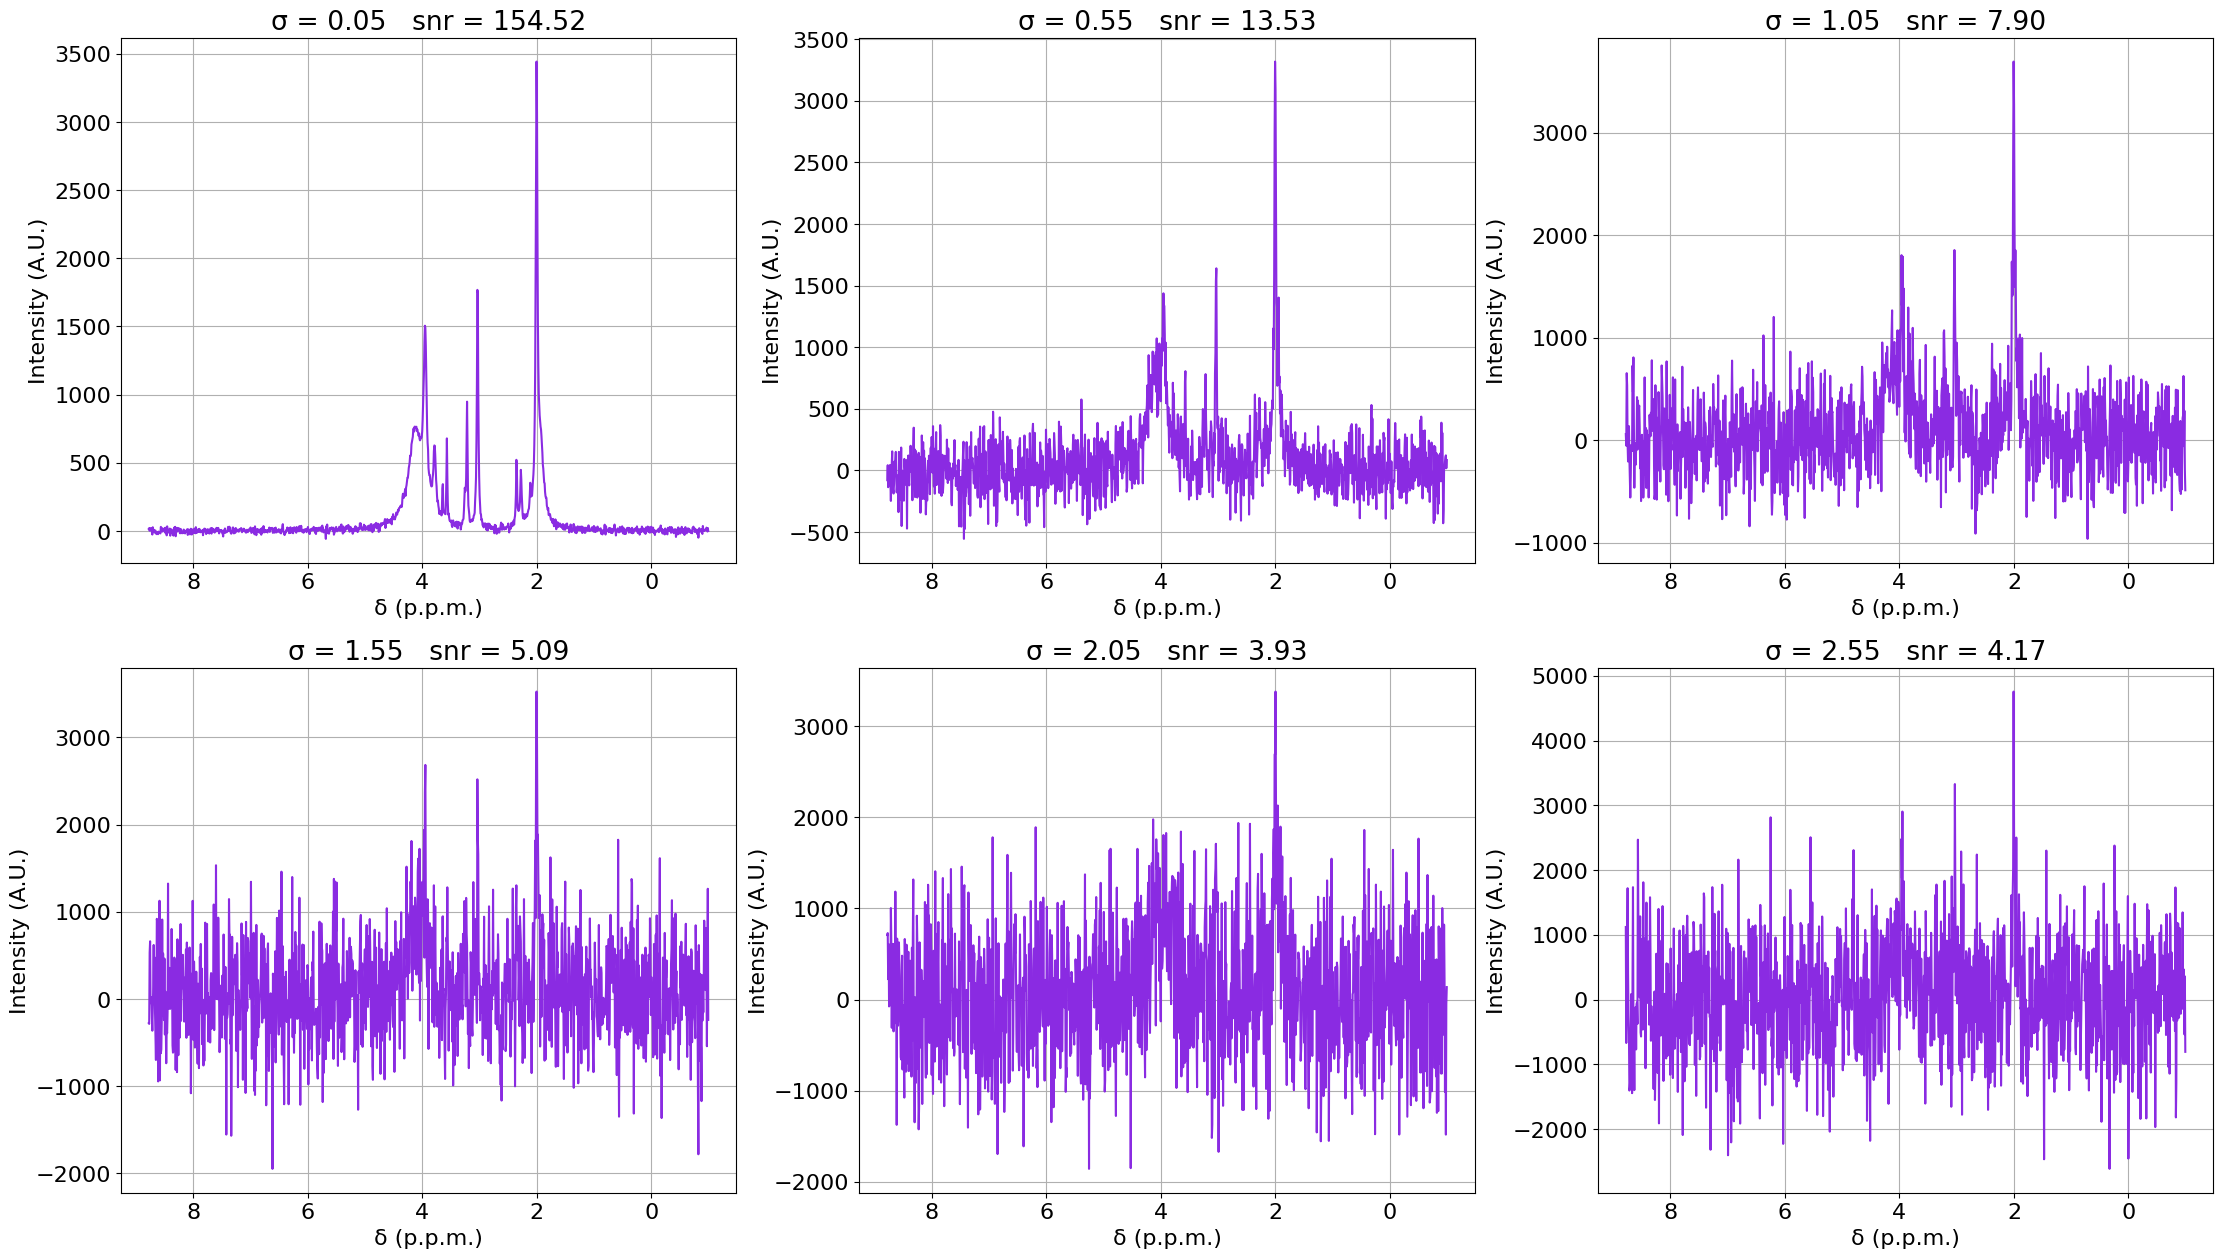
\includegraphics[scale=0.22]{snr_limits.png}
    \centering
    \caption{Limites de validade do desvio padrão.}
    \label{fig:9}
\end{figure}

Em seguida, foram gerados um conjunto de $50$ sinais utilizando os parâmetros correspondentes aos metabólitos na \autoref{table:1}, corrompidos por ruídos gaussianos com desvios padrão variando dentro dos limites definidos, com um intervalo de $0.1$ entre cada, $1000$ vezes. Cada sinal variava 
entre o intevalo temporal de $[0.0, 1.0)$ segundos, com uma frequência de sampling de $100000$ pontos por segundo, resultando em $100000$ pontos. 

Muito embora a quantidade de pontos não seja compatível se comparada a um sinal clínico com um número significativamente menor de pontos, dado o interesse do presente trabalho de avaliar a relação entre os desvios padrão, optou-se por essa quantidade afim de melhorar a qualidade da análise.

Para cada vez, foi calculado seu espectro, e para cada espectro foi calculado o desvio padrão resultante, que por sua vez contribuiu para o cálculo do desvio padrão 
resultante médio de cada sinal corrompido. Por meio da \autoref{eq:2}, com o pico normalizado como descrito anteriormente para $1$, foi também possível calcular qual seria o SNR médio resultante.

\begin{figure} [H]
    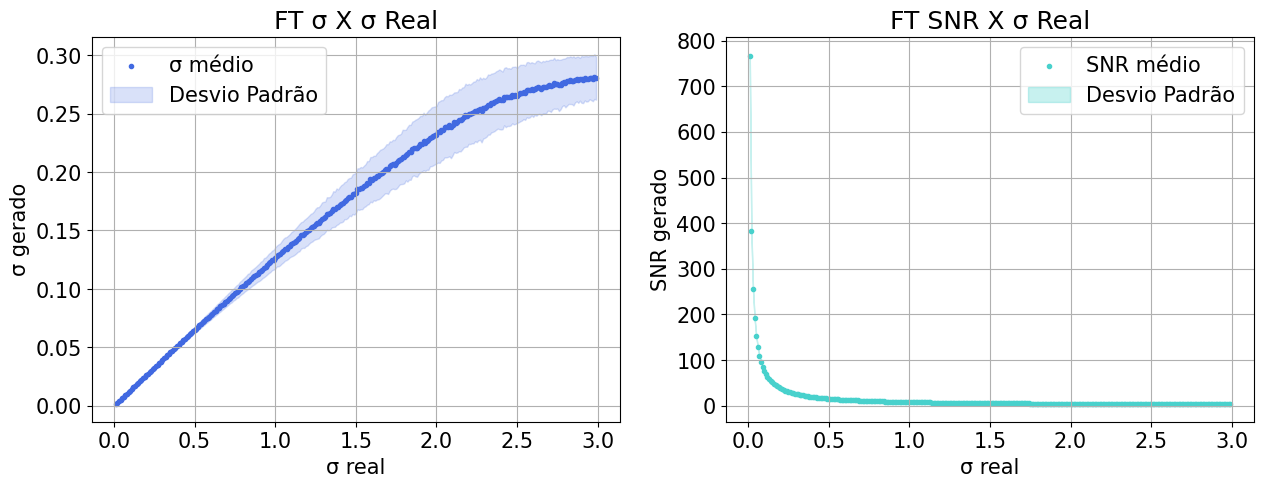
\includegraphics[scale=0.37]{evolucao-sigmas.png}
    \centering
    \caption{Evolução do $\sigma$ gerado com relação ao $\sigma$ utilizado para a geração do ruído.}
    \label{fig:6}
\end{figure}

Pela \autoref{fig:6}, verifica-se que o desvio padrão resultante parece ter uma relação não linear com o desvio padrão usado na geração. Partindo do pressuposto que a relação se assemelha a uma função exponencial, a \autoref{eq:9} foi utilizada como modelo para o ajuste dos dados. É importante ressaltar que 
$a$ e $c$ são constantes, e $b = \ln(a)$ de maneira a garantir que no zero a função, assim como os dados indicam, seja também zero.

\begin{equation} \label{eq:9}
    SNR(\sigma) = a - e^{b - c\sigma} 
\end{equation}

O ajuste foi feito em 20 conjuntos de médias diferentes, resultando em um $a = (0.494 \pm 0.002)$ e $c = (0.306 \pm 0.002)$. Com os parâmetros calculados e a partir da relação \autoref{eq:2}, foi criada uma função que, a partir de um valor de entrada de SNR, estima um valor aproximado para qual deve ser o desvio padrão a ser usado para 
gerar o ruído a corromper o sinal real de maneira a atingir o SNR desejado.

\begin{equation} \label{eq:10}
    \sigma (SNR) = \frac{log(a) - log(a - \frac{1}{SNR})}{c}
\end{equation}

Essa função foi então testada a fim de garantir sua acurácia na predição dos desvios padrão. Como pode ser conferido pela \autoref{fig:7}, o sigma resultante gerou sinais cujos SNR dos espectros difere dos SNR desejados, com um erro que cresce linearmente com o SNR.

\begin{figure} [H]
    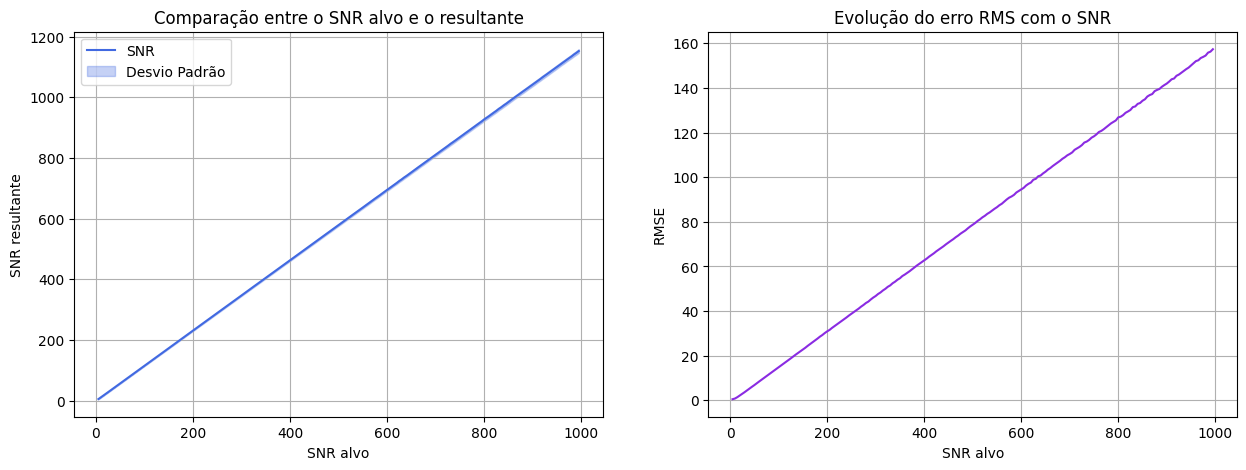
\includegraphics[scale=0.4]{evolucao-rmse-errado.png}
    \centering
    \caption{Evolução do RMSE gerado com relação ao SNR requisitado.}
    \label{fig:10}
\end{figure}

Apesar de os valores resultantes serem diferentes, sua relação ainda parecia ser linear. 
Foi feita então uma segunda correção, ajustando uma curva à reta que relaciona o SNR alvo com 
o resultante de maneira a prever qual seria sua relação, utilizando a \autoref{eq:12}.

\begin{equation} \label{eq:12}
    SNR_{resultante} = a SNR_{alvo} + b    
\end{equation}
Essa correção permitiria ajustar o SNR alvo de maneira a encontrar o valor na reta que de 
fato correspondesse ao valor requisitado. Esse ajuste gerou uma reta com parâmteros 
$a = (0.1591 \pm 0.0001)$ e $b = (-1.00 \pm 0.03)$.
\begin{figure} [H]
    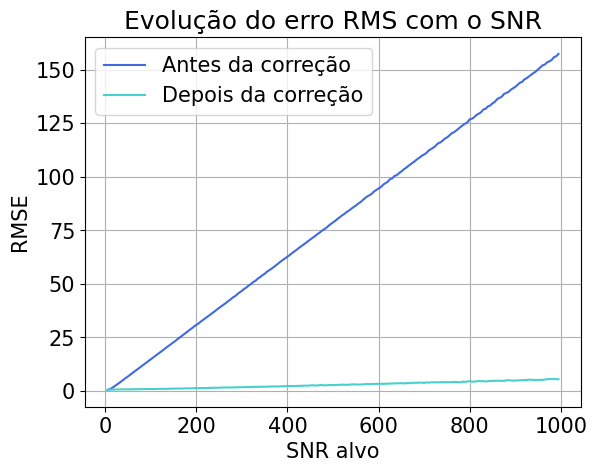
\includegraphics[scale=0.5]{evolucao-rmse.png}
    \centering
    \caption{Evolução do RMSE gerado com relação ao SNR requisitado após a correção.}
    \label{fig:8}
\end{figure}

\begin{figure} [H]
    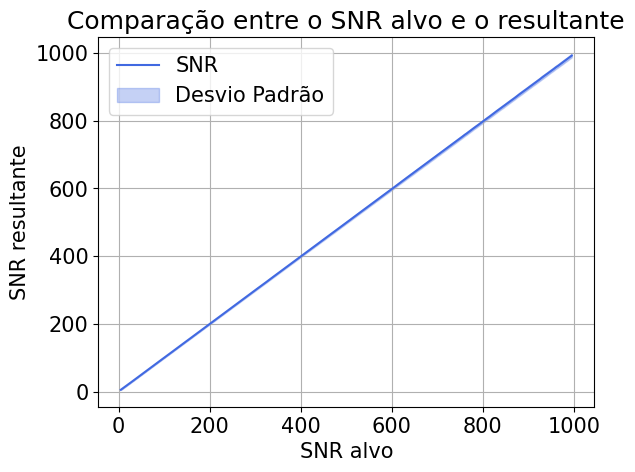
\includegraphics[scale=0.5]{SNR_pos_correcao.png}
    \centering
    \caption{Evolução do SNR resultante após a correção.}
    \label{fig:11}
\end{figure}

Após essa correção, a função de predição foi novamente testada, agora com os parâmetros de ajuste da reta.
Como pode ser conferido pela \autoref{fig:8}, o erro dos SNRs resultantes após a correção foi 
significativamente menor, chegando à casa de poucas unidades para os valores mais altos. Como também explicitado pela \autoref{fig:11}, esse resultado 
demonstrou uma capacidade de predição relevante do sigma necessário para valores de SNR requisitados, permitindo assim 
a predição de um $\sigma$ de entrada na função de corrupção do sinal a partir de um valor de SNR desejado. 

\subsection{Próximas Etapas}

Apesar de o cronograma apresentado na \autoref{sec:cronograma} estipular o estudo do algoritmo de MPM para o segundo semestre,
uma mudança foi feita durante o andamento dessa etapa inicial do projeto. Foi antecipada a parte da caracterização do ruído para o segundo semestre, e adiado o estudo do MPM 
para o terceiro, de maneira a desenvolver uma fundamentação da simulação de espectros mais robusta e polida, a fim de mitigar o surgimento de problemas em etapas subsequentes.

Feita essa consideração, a próxima etapa do projeto será de estudo do algoritmo de MPM, dando prosseguimento às etapas remanescentes, como explicitadas anteriormente.

\subsection{Conclusão}

A partir do estudo da relação entre desvios padrão e o SNR resultante, 
foi verificada uma relação linear para valores baixos de sigma, e uma 
saturação para valores mais altos. Também foram calculados 
parâmetros de ajuste dos dados, com os quais foi feita a correção dos 
valores de SNR de entrada, viabilizando a dedução de uma função que 
relacionasse diretamente $\sigma$ e SNR com uma margem de erro 
relativamente baixa para as intenções do projeto. 

Dessa maneira, foi obtido um nível de controle maior sobre os parâmetros da simulação dos sinais de RM, etapa essencial para 
garantir a qualidade do estudo da aplicação do MPM nos mesmos.

\bibliographystyle{plain}
\bibliography{../refs}

\section{Produção no Período}

Durante o período, foi feita participação na Semana da Física do Instituto de Física de São Carlos (IFSC),
que contou com apresentação de posteres.

\end{document}